\documentclass[11pt]{article}

\usepackage{tls}


\title{Title of your TLS paper}
\author{Beatrice McHuggins and Harold Q. Snodgrass}
\organization{University of Texas at Austin}

\begin{document}

\maketitle

\section{Introduction}

The following rules apply to all submitted papers:

\begin{itemize}
\item they must be written in English
\item they must contain the name(s) of the author(s)
\item the maximum length is twenty (20) pages 
\item they must be submitted in PDF format (please make sure everything renders
appropriately before you send in your document)
\end{itemize}

This paper template can be found on the conference website. Please use either
the Microsoft Word compatible file or the \LaTeX\ format file when preparing
your submission. If there are special questions or wishes regarding paper
preparation and submission for TLS 14, correspondence should be addressed via
email to {\tt tls.conference@gmail.com}; please include {\em ``Paper submission; TLS 14''} 
in the subject line of the email.

%Information for full paper submission will be available on the web at:

%\url{http://humanities.uchicago.edu/orgs/cls} 

%\noindent
%under which you also will find instructions for paper preparation and usage of templates.

\section{Page layout and style}

The page layout should conform to the following rules. By far the easiest way
to meet these requirements is to use the supplied templates (Word or \LaTeX)
and check details against this example file. If for some reason you cannot use
Word or \LaTeX, please follow these rules as carefully as possible, or contact
the editors at {\tt tls.conference@gmail.com} for further instructions.

\subsection{Basic layout features}
Please adhere to the following basic layout features:
\begin{itemize}
\item Page format should be US Letter.
\item Left and right margins are 1.5''.
\item Top and bottom margins are 1.25''.
\item The header and footer should be left empty; they will be added later.
\item Check indentations and spacings by comparing with this example file.
\end{itemize}

\subsubsection{Headings}

Section headings (including sub-headings and sub-sub t headings) are left
justified in boldface with the first letter capitalized and the rest of the
heading in lower case. See examples in this file. No more than 3~levels of
headings should be used.

\subsection{Text font}

11~point Times or Times New Roman font is used for the main text. Other font
types may be used if needed for special purposes. If you are using special fonts
such as SIL IPA or Arboreal, please advise us which fonts you have made use of,
and include them with your submission. When making the final PDF file, remember
to \textit{embed all fonts}!

\subsection{Figures}

All figures should be centered on the page. Figure captions should follow each 
figure and have the format given in Fig.~\ref{fig:vowels}.\\

\begin{figure}[!ht]
\begin{center}
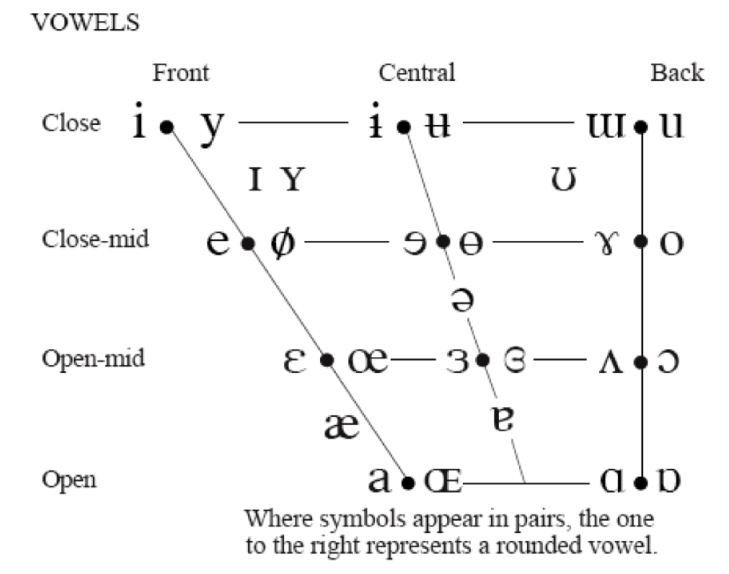
\includegraphics[width=10cm]{ipa}
\caption{The vowel chart used in the International Phonetic Alphabet (IPA).}\label{fig:vowels}
\end{center}
\end{figure}

Figures should preferably be line drawings. If they contain grey shades, it
should be checked that they print well on a high-quality noncolor laser printer.
Color figures should not be used.


\subsection{Interlinear glosses}

How you keep your glosses lined up properly depends on the software you are
using. If you are using Word, please insert your glosses inside a table, with
the borders of the table set to ``none'' so that they are not visible. If you
are using \LaTeX\, we recommend the \texttt{$\backslash$gll} function of
\texttt{gb4e.sty}.

\begin{exe}
\ex
\gll \textit{Los} \textit{niños} \textit{le} \textit{molestan}\\
the-{\sc pl} children {\sc dat} bother\\
\trans `Children irritate him.'
\end{exe}



\subsection{Tables}

An example of a table is shown as Table~\ref{tab:decibel}.  Somewhat different
styles are allowed according to the type and purpose of the table. Color should
not be used, but grey shading is allowed. There should be a margin of 6~points
(pt) above and below the table. The caption text may be above or below the
table, but this should be consistent throughout the submission.\\% Left and right indentation of the caption should be 0.5~cm.

\begin{table}[h]
\centering
\begin{tabular}{|c|c|}
\hline
\rowcolor[gray]{.75}
\hline
ratio    & Decibels\\
\hline
$1/1$    & $0$\\
$2/1$    & $6$\\
$3.16$   & $10$\\
$1/10$   & $-20$\\
$10/1$   & $20$\\
$100/1$  & $40$\\
$1000/1$ & $60$\\
\hline
\end{tabular}
\label{tab:decibel}
\caption{This is an example of a table showing Decibel (dB) ratios.}\label{tab:decibel}
\end{table}

\subsection{Examples}

If you are using Word, please insure that your example numbers are consistent
with your text references. If you are using \LaTeX\, we recommend using the
\texttt{gb4e} package. It's not perfect, but it allows for sub-examples,
functionality not supported by the \texttt{equation} environment.

\begin{exe}
\ex\label{ex1} \begin{xlist}
        \ex\label{ex1a} This is an English example.
        \ex\label{ex1b} This is a longer English example.
    \end{xlist}
\ex\label{ex2} Here is a free-standing example.
\end{exe}

Example (\ref{ex1}) contains two sub-examples: (\ref{ex1a}) and (\ref{ex1b}).

\subsubsection{Equations}

If you are using \LaTeX\, please do {\bf not} use the \texttt{equation} macros,
as they use an internal numbering order that does not interact with
\texttt{gb4e}! To get into math mode, use the \$ ... \$ delimiters. 

\begin{exe}
\ex 
$t_0 = \frac{1}{f_0}$
\end{exe}

\subsection{Page numbering}
Page numbers will be added electronically to the document later. \textit{Please
do not add page numbers and please do not make any footers or headers!}

\subsection{Submission length}
Submissions must not exceed 20 pages, including data and references. 

\subsection{OT tableaux}
If using Word, OT tableaux should be implemented as standard tables. If using 
\LaTeX\, OT tableaux should be implemented within the standard \texttt{tabular}
environment. If you wish to make use of any other packages, such as
\texttt{arydshln}, please include the style file when submitting your paper.

\begin{exe}
\ex 
\begin{tabular}
       {|lc|c|c|c|}\hline   
      & \textbf{input}  & {\sc Can_{1}} &  {\sc Can_{2}} & {\sc Can_{3}} \\ \hline\hline
    	\hand  & \textit{candidate a}     &           &   *        &\cellcolor{lightgray} *         \\ \hline
      		  & \textit{candidate b}      &           &  *!       &\cellcolor{lightgray}          \\ \hline
		  & \textit{candidate c}    & *!        &\cellcolor{lightgray}         &\cellcolor{lightgray}        \\ \hline
\end{tabular}

\end{exe}

\subsection{Phonetic fonts}

You can use phonetic symbols and special characters in your paper. To make sure
that readers of your article can see the phonetic symbols in the PDF document
all special symbols must be embedded in the PDF. Depending on the software you
use to produce the PDF (see Section~3) the details may vary. In our experience
the fonts are usually embedded, but this can be checked e.g. by inspecting the
``Document Properties -- Fonts'' in Acrobat Reader.

For \LaTeX\ users, we recommend the \texttt{tipa} package to render phonetic
fonts; it is available at CTAN. If you are using Word, please remember to
include the font package with your Word document.


\subsection{Syntactic trees}
Microsoft Word users should be sure to include any special fonts used to
generate syntactic trees, where “special” is defined as “not included as
part of the standard MS Word distribution”. For \LaTeX\ users, we recommend
the \texttt{qtree} package.


\begin{exe}
\ex \Tree [.IP [ Roses ].NP_i [.I\1 [ are ].I^0 
        [.VP t_i [ [ going ].V^0 \qroof{out of style}.PP ].V\1 ].VP 
          ].I\1 ]

\end{exe}


\subsection{References}

Please use LSA style: name (year or (Name year). Formulations
with author names like ``\ldots\ as \namecite{Ladefoged:2003}
showed that \ldots'' are acceptable, but not ``as shown in [Ladefoged,
2003]'' or ``as shown in (Ladefoged~[6])''. See Section 4 for more on references.

\subsection{Hyperlinks}

Links to URLs or email addresses should be formatted as normal text,
\textit{not} as hyperlinks and not blue or underlined etc. Usually hyperlinks to
web pages are listed in the references section (e.g. \citeboth{Praat}). If
required, line breaks can be placed within URLs after slashes or dashes, but
double check that no hyphens are inserted.

\subsection{Footnotes}

This is an example of a footnote\footnote{Remember that these are footnotes, not
places to go off on multi-paragraph rants.}.


\section{PDF details}

PDF files submitted must comply with the following requirements:

\begin{enumerate}
\item all special fonts and symbols must be embedded in the PDF file
so that correct rendering of the PDF does not depend on the fonts
installed on the viewer's computer
\item there must be no password protection on the PDF file, i.e.\ PDF
files must not be protected by PDF security in any way (e.g.\ content
extraction, document assembly, highresolution printing etc.\ must not
be forbidden)
\item PDF files should not contain any colors, hyperlinks, multimedia
or 3D content, JavaScript, or forms
\end{enumerate}


\section{Format of references}

Monographs such as \namecite{Fant:1960} consist of author(s) last name(s),
initial of the first name(s), year of publication, title in italics, location of
the publication, and publisher. The names of multiple authors are separated by
commas listed in the sequence last name, comma, initial(s) of the first name(s)
(cf.\ the examples~\citeboth{Beattie/etal:1982},
\citeboth{Peterson/Barney:1952}).

Contributions to volumes, e.g.~\namecite{Stevens:1999}, follow the
convention that the title of the volume is in italics, but not the
title of the contribution. Book editors should appear after the book title, 
followed by page numbers, place of publication, and publisher.

Journal articles should be handled in the same way as contributions to
volumes, except that the title of the journal is in italics and
the editors are not listed. Longer names of well-known journals can be
abbreviated (e.g.~\citeboth{Peterson/Barney:1952}).

Articles in conference proceedings such as \namecite{Ladefoged:2003} are
referenced in the same way as journal articles.  The word
\textit{proceedings} can be abbreviated and the location should be
mentioned after the name of the conference. Here, abbreviations of
well-known conferences are possible.

\bibliographystyle{tlslike}
\bibliography{tls}

\end{document}

